\documentclass{journal}
\usepackage{graphicx}	% package for using graphics
\usepackage{float}	% package for positioning figures
\usepackage[left=1.5 in,top=1 in,right=1.5 in,bottom=1 in]{geometry} % Document margins
\usepackage[backend=biber, style=alphabetic, sorting=ynt]{biblatex} % package for creating bibliography

\addbibresource{references.bib}

\title{DESIGNING AN OPTIMIZED AIRFRAME}

\author{Nathan Pettit}


\begin{document}
	
	\maketitle	
	\section{Introduction}
	This report covers the research done in learning how airframes work, specifically how the shape of the airfoil affects airfoil polar, how the shape of the airframe affects airfoil polar, and how the efficiency of the airframe is related to all of this. The knowledge gained from this research was then used to design an airframe to solve a real world problem.\\
	
	\section{Airfoil Design}
	This section reviews research done on airfoils. There are 5 areas that are covered in this research. First, it explores the effect of airfoil angle of attack on lift, drag, and moment. Second, it compares data collected by Xfoil to experimental data. Third, it explores the effect of different Reynolds numbers on airfoil polar. Fourth, it explores the effect of airfoil thickness. And fifth, it explores the effect of airfoil camber.\\
	
	\subsection{Methods}
	The airfoil research was done by writing a program in the Julia language that used the Xfoil.jl library \cite{McDonnell}. In order to explore the effect of angle of attack, Reynolds number, thickness, and camber on the airfoil polar, Xfoil's solve\_alpha() function was used, so that the coefficients of lift, drag, and moment could be used for comparison. For the Reynolds number, thickness, and camber comparisons, their coefficients vs. angles of attack plots were compared. This way, trends could be seen and they could be compared effectively.
	
	\subsection{Results}
	One of the most stressed parts of this research was seeing how different airfoil angles of attack affected the lift, drag, and moment on the airfoil. In order to see those relationships, only the coefficients of drag, lift, and moment needed to evaluated, rather than the moment and the forces of lift and drag. This is because those coefficients are dimensionless numbers. Figure \ref{fig:aoa-coefficients} shows the relationships between lift, drag, and moment and \(\alpha\) for a NACA 2412 airfoil.\\
	
	\begin{figure}[H]
		\centering
		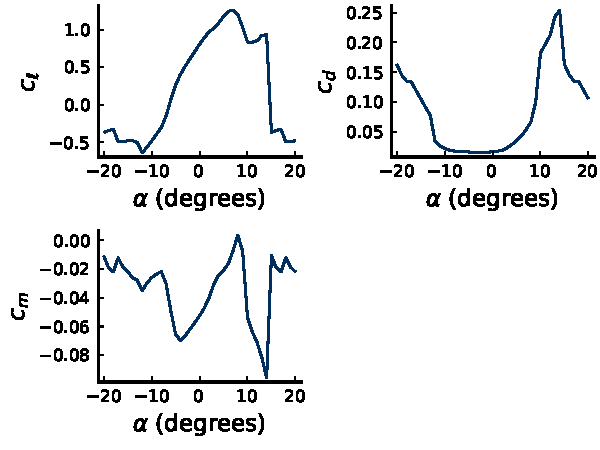
\includegraphics{../graphics/aoa-coefficients.pdf}
		\caption{\emph{The coefficients of lift, drag, and moment plotted against angle of attack for a NACA 2412 airfoil.}}
		\label{fig:aoa-coefficients}
	\end{figure}
	
	The coefficients of lift (\(c_\ell\)) and drag (\(c_d\)) both increase as angle of attack (\(\alpha\)) increases, because as the angle increases, the pressure differential between the top and bottom of the airfoil becomes larger. This also increases coefficient of moment (\(c_m\)). It is also important to note that figure \ref{fig:aoa-coefficients} establishes that lift is negative when \(\alpha\) is less than zero, which makes sense because the pressure differential goes from having greater pressure on the bottom (positive lift) to greater pressure on the top of the airfoil (negative lift). It can also be seen that the zero-lift angle of attack is somewhere between 0 and 0.5 degrees, which is where the lift changes from negative to positive. It appears that stall takes place at an angle of attack of about 10 degrees, which is where the angle of attack becomes too great for the airfoil to produce lift. This can be clearly seen on the lift and drag plots.\\
	
	In order to see the accuracy of Xfoil, the results gained from Xfoil were plotted against experimental data from a study done on the NACA 2412 airfoil (see figure \ref{fig:airfoil-comparison}).\\
	
	\begin{figure}[H]
		\centering
		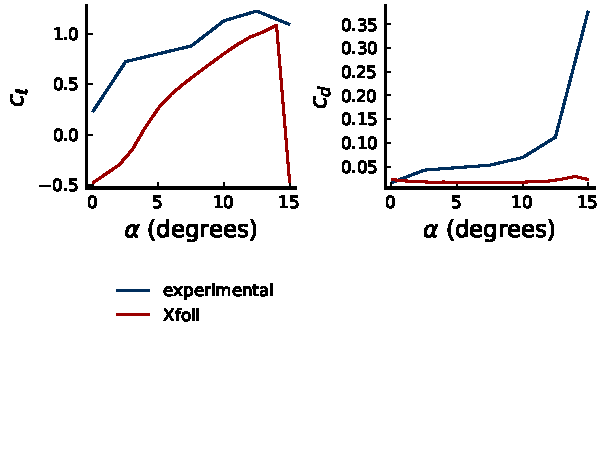
\includegraphics{../graphics/airfoil-compare.pdf}
		\caption{\emph{The comparison of data collected experimentally to data collected from Xfoil.}}
		\label{fig:airfoil-comparison}
	\end{figure}
	
	It is interesting to see that the experimental lift curve looks very similar to the one obtained from Xfoil, except shifted up. Also, the drag curves between experimental and Xfoil are very different. The reason for this is unknown, although it might be an error in Xfoil calculations.\\
	
	Next to be evaluated was how varying the Reynolds number affects the airfoil polar. The purpose of the Reynolds number is to compare inertial forces to viscous forces. It is an indicator of how viscous the fluid that an airfoil is traveling through is. A high Reynolds number is an indicator that fluid flow will be turbulent, where as a low Reynolds number is an indicator of laminar flow. In figure \ref{fig:altered-reynolds}, the relationships between Reynolds number and the coefficients are shown.\\
	
	\begin{figure}[H]
		\centering
		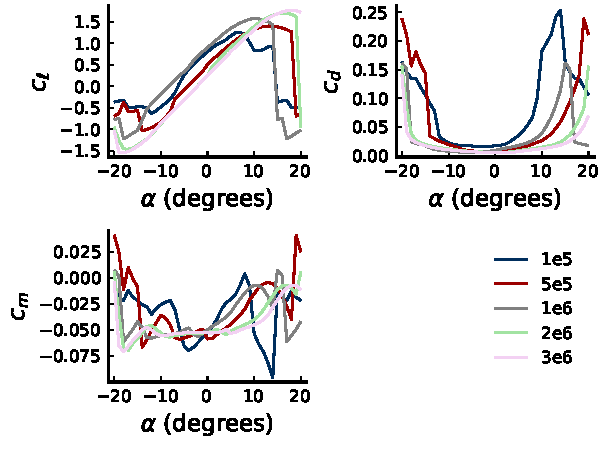
\includegraphics{../graphics/altered-reynolds.pdf}
		\caption{\emph{The lift, drag, and moments against angle of attack for varying Reynolds numbers.}}
		\label{fig:altered-reynolds}
	\end{figure}
	
	As the Reynolds number increases, it seems that all the curves become more smoothed out. Also as the Reynolds number increases, the curves of drag and moment become more leveled out. These results make logical sense, because changes in how turbulent the flow is doesn't affect the lift generated as much. On the other hand, higher Reynolds numbers and therefore more turbulent flow decreases the drag and moment at more extreme angles of attack (see figure \ref{fig:altered-reynolds}). The reason for all of this is higher Reynolds numbers means that the fluid flow around the airfoil doesn't have as much of an effect on it. This is also why the curves seem to converge as the Reynolds number increases.\\
	
	As for physical attributes of the airfoil, its thickness and camber were changed to see their effect. The thickness of an airfoil is the greatest distance between the upper and the lower surfaces of an airfoil. In figure \ref{fig:altered-thickness}, the relationship between airfoil thickness and the coefficients of lift, drag, and moment can be seen.\\
	
	\begin{figure}[H]
		\centering
		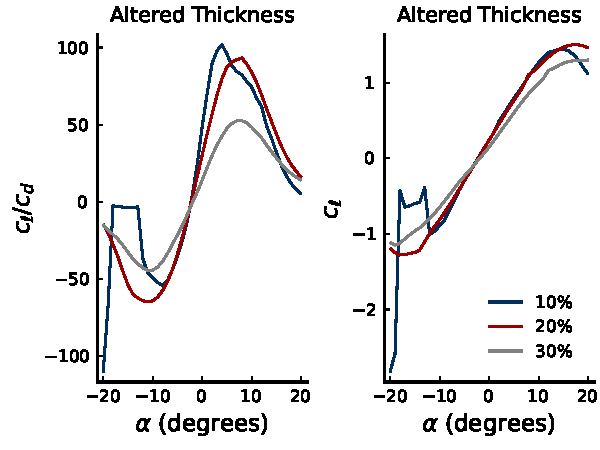
\includegraphics{../graphics/altered-thickness.pdf}
		\caption{\emph{The ratio of lift to drag coefficients and coefficient of lift against angle of attack.}}
		\label{fig:altered-thickness}
	\end{figure}
	
	As the thickness of the airfoil increases, the ratio of lift to drag curve becomes more shallow. This is because increasing thickness leads to lift and drag becoming closer and closer to each other. It is interesting to see though that no matter the thickness, the zero lift angle of attack remains the same (see figure \ref{fig:altered-thickness}).\\
	
	The camber of an airfoil is the measure of the asymmetry between the two acting surfaces of an airfoil. An airfoil with zero camber is symmetric. In figure \ref{fig:altered-camber}, the effect of different cambers can be seen.\\
	
	\begin{figure}[H]
		\centering
		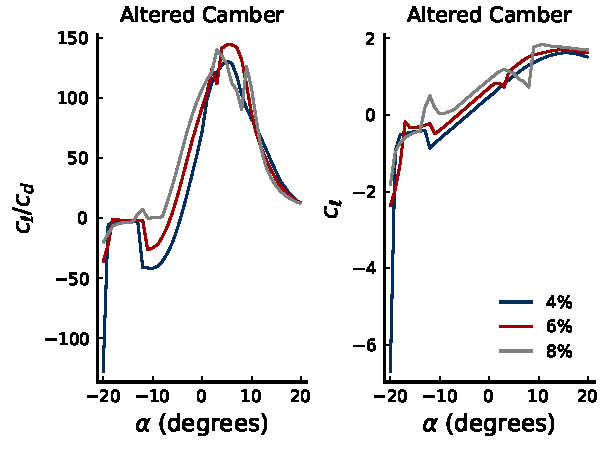
\includegraphics{../graphics/altered-camber.pdf}
		\caption{\emph{The ratio of lift to drag coefficients and coefficient of lift against angle of attack.}}
		\label{fig:altered-camber}
	\end{figure}
	
	As the camber of the airfoil increases, the lift to drag ratio becomes higher and the whole curve is shifted upwards. This also happened with the coefficient of lift. This also means that the zero lift angle of attack became greater with increasing camber.\\
	
	\section{Airframe Analysis}
	
	This section covers research done on airframes, specifically how aspect ratio and efficiency are related, how tail volume ratios affect stability derivatives, and how angle of attack affects the lift coefficient. The results of this research came from evaluating airframes using VortexLattice.jl \cite{McDonnell-Ning}.\\
	
	\subsection{Methods}
	The VortexLattice.jl library \cite{McDonnell-Ning} was used to evaluate airframes. Specifically, the steady\_analysis() function was used to perform steady state analysis on the airframe, the body\_forces() function was used to find the near-field forces acted on the airframe, and the stability\_derivatives() function was used to find the stability derivatives of an airframe system.

	\subsection{Results}
	
	In order to see the relationship between aspect ratio and the efficiency, the inviscid span efficiency (see equation \ref{eqn:efficiency}) was calulated for airframes with aspect ratios (see equation \ref{eqn:aspect-ratio}) ranging from 3 to 15.\\
	
	\begin{equation}
		e_{inv} = \frac{C_L^2}{\pi{ARC_D}}
		\label{eqn:efficiency}
	\end{equation}
	
	\begin{equation}
		AR = \frac{b}{c} = \frac{b^2}{S_{ref}}
		\label{eqn:aspect-ratio}
	\end{equation}
	
	After the program calculated the efficiency, it produced a plot shown in figure \ref{fig:efficiency}.\\
	
	\begin{figure}[H]
		\centering
		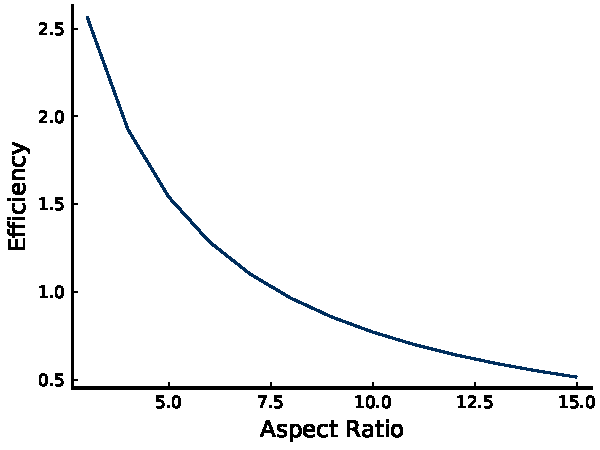
\includegraphics{../graphics/efficiency.pdf}
		\caption{\emph{The relationship between aspect ratio and inviscid span efficiency.}}
		\label{fig:efficiency}
	\end{figure}
	
	In reality, figure \ref{fig:efficiency} doesn't show a relationship that is actually interesting, but it does mathematically plot it correctly. It is simply the definition of inviscid span efficiency.\\
	
	Another characteristic of these airframes that was observed was their stability derivatives. Stability derivatives were calculated for airframes with different tail volume ratios, both vertical and horizontal. The definitions of those ratios are equations \ref{eqn:vtail-ratio} and \ref{eqn:htail-ratio}. Airframes were evaluated with vertical tail volume ratios that varied from 0.001 to 0.0156 and horizontal tail volume ratios that varied from 0.001 to 0.1458. Those bounds were chosen because all airframes that have tail volume ratios between them have reallistic dimensions.\\ 
	
	The stability derivatives that are affected by a change in vertical tail volume ratio are \(C_{\ell{b}}\) and \(C_{nb}\). \(C_{\ell{b}}\) is the stability derivative associated with roll stability. \(C_{nb}\) is the stability derivative associated with yaw stability. An airframe is stable if \(C_{\ell{b}}\) is less than 0 and \(C_{nb}\) is greater than 0.\\
	
	\begin{equation}
		V_v = \frac{l_vS_v}{Sb}
		\label{eqn:vtail-ratio}
	\end{equation}
	
	\begin{equation}
		V_h = \frac{l_tS_t}{SC_{ma}}
		\label{eqn:htail-ratio}
	\end{equation}
	
	In figure \ref{fig:vtail-stability} , we can see that the airframe is stable for vertical tail volume ratios greater than 0.003, but it becomes unstable when the ratio is less than 0.003, at around 0.002. The stability derivatives that are affected by a change in horizontal tail volume ratio are \(C_{La}\) and \(C_{ma}\). An airframe is stable if \(C_{La}\) is greater than 0 and \(C_{ma}\) is less than 0. Figure \ref{fig:htail-stability} shows that the airframe is stable for horizontal tail volume ratios greater than 0.05, but becomes unstable when the ratio is less than 0.05, at around 0.025.\\
	
	\begin{figure}[H]
		\centering
		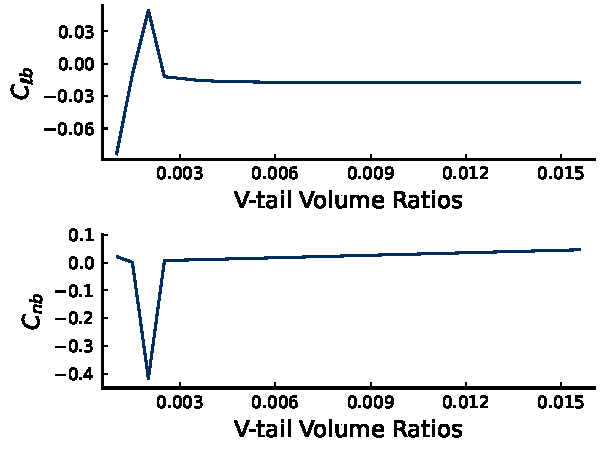
\includegraphics[scale=0.73]{../graphics/vtail-stability.pdf}
		\caption{\emph{This diagram shows the relationship between vertical tail volume ratio, \(C_{\ell{b}}\), and \(C_{nb}\).}}
		\label{fig:vtail-stability}
	\end{figure}
	
	\begin{figure}[H]
		\centering
		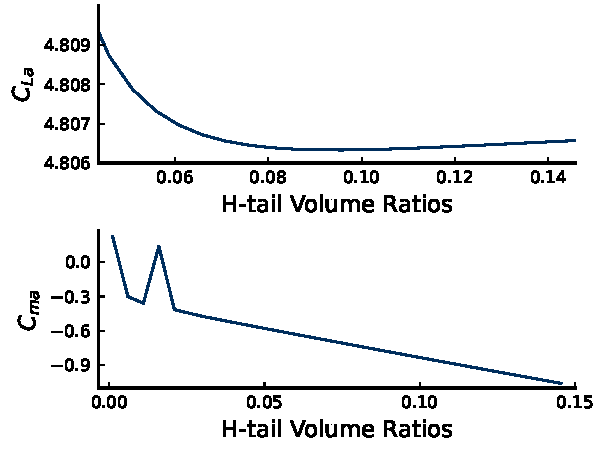
\includegraphics[scale=0.73]{../graphics/htail-stability.pdf}
		\caption{\emph{The relationship between horizontal tail volume ratio, \(C_{La}\), and \(C_{ma}\).}}
		\label{fig:htail-stability}
	\end{figure}
	
	In previous research about airfoils, I found that as angle of attack increases, the lift coefficient also increases, up to a certain point. At that point, the lift coefficient sharply drops, and this is where stall takes place. In that previous research, Xfoil.jl \cite{McDonnell} was used to calculate the lift coefficient for varying angles of attack. A relationship between angle of attack and lift was also tried to be found here, but instead of using Xfoil.jl \cite{McDonnell}, VortexLattice.jl \cite{McDonnell-Ning} was used. A plot was produced showing the relationship between angle of attack and lift (see figure \ref{fig:aoa-lift}).\\
	
	\begin{figure}[H]
		\centering
		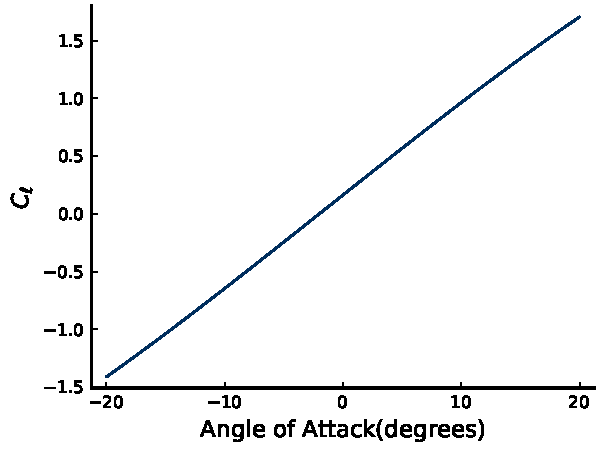
\includegraphics{../graphics/aoa-lift.pdf}
		\caption{\emph{The relationship between angle of attack and lift for an airframe.}}
		\label{fig:aoa-lift}
	\end{figure}
	
	In comparison to the plot created using Xfoil.jl \cite{McDonnell} (see figure \ref{fig:aoa-coefficients}), figure \ref{fig:aoa-lift} looks very similar between angles of attack of -10 and 10. However, past those angles of attack is where it differs. In the Xfoil plot, it shows very clearly where stall would take place, but in this VortexLattice plot, the plot continues linearly and never drops off, never indicating stall. This is why the Vortex Lattice method is not always a great choice for investigating airframes. It is only accurate when the angle of attack is small, because it assumes that the flow is inviscid at all angles of attack. This is why in figure \ref{fig:aoa-lift} it looks very linear and does not indicate where stall would take place, where as the Xfoil plot does.\\
	
	\section{Airframe Aerodynamic Design}
	
	This section discusses the designing of an airframe that can lift 0.5 kilograms, has a wingspan no greater than 1.5 meters, and is stable. In doing this, research done previously was employed as well as knowledge gained from that research.\\
	
	\subsection{Methods}
	The results of this research came from evaluating potential airframe solutions using VortexLattice.jl \cite{McDonnell-Ning}. In order to optimize the airframe, the process, discussed in the introduction to "Engineering Design Optimization" by Joaquim R.R.A. Martins and Andrew Ning, was followed. The objective function  that was minimized was the equation used to calculate the velocity needed to produce the necessary lift to carry 0.5 kilograms (see equation \ref{eqn:needed-velocity}).\\
	
	\begin{equation}
		V = \sqrt{\frac{L}{(0.5)(C_L)(\rho)(S_{ref})}}
		\label{eqn:needed-velocity}
	\end{equation}
	
	\begin{itemize}
		\item \(L\) - the lift needed to takeoff with 0.5 kilograms, in this case 4.905 N
		\item \(\rho\) - the density of the air (1.225 \(kg/m^3\))
		\item \(S_{ref}\) - the reference area, in this case the wing area
	\end{itemize}
	
	The design variables that were altered in order to minimize that function was the mean aerodynamic chord length of the wing and the length from wing to tail on the airframe. The reason I chose these design variables was because I knew that the airframe that would generate the most lift would have the max wingspan possible (so in this case 1.5 m), and so altering the chord length would help me find the wing that needed the least speed to takeoff. I also chose the length from wing to tail as a design variable because I knew altering it would change how stable the airframe was.\\
	
	However, as I worked with these design variables, it was discovered that the greater the length from wing to tail, the more stable the airframe. For this reason, I put an upper limit on that length to be 2.0 m, so that the found airframe would be realistic. I also put a constraint on the aspect ratio of the wing, which was that it had to be greater than 2.0. The way that I found the optimal airframe was I changed those design variables together, so that it found the airframe that took off at the least velocity, but was the most stable. The efficiency of the airframe with different wing taper ratios was also evaluated by plotting the lift coefficient distribution against the optimal distribution, which was a ellipse. The ideal taper ratio was the one that produced a lift coefficient distribution closest to that elliptical distribution. This was done so that the final airframe design not only optimized my objective function, but was also the most efficient design.\\
	
	\subsection{Results}
	
	After running the optimize\_airframe() function, it found that the most optimized airframe was one that had the following characteristics (figure \ref{fig:ideal_design} shows what the design looks like):
	
	\begin{figure}[H]
		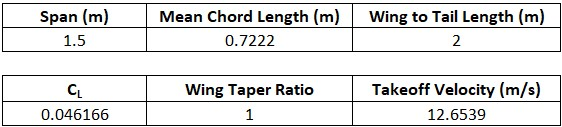
\includegraphics{../graphics/ideal_attributes.jpg}
		\label{fig:ideal_attr}
	\end{figure}
	
	\begin{figure}[H]
		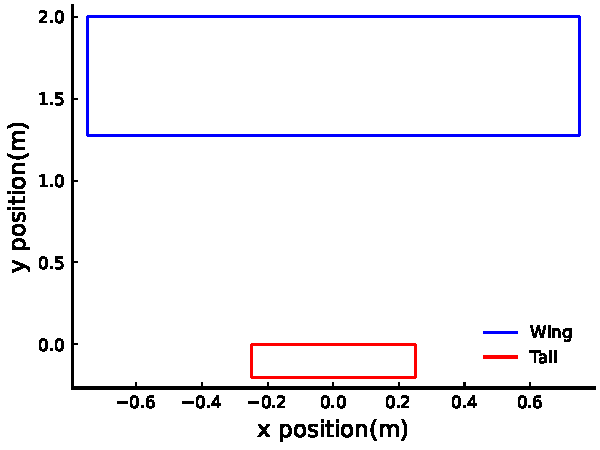
\includegraphics{../graphics/ideal_design.pdf}
		\caption{\emph{The design of the optimized airframe.}}
		\label{fig:ideal_design}
	\end{figure}
	
	The aforementioned necessary lift was 4.905 Newtons. This number was found by multiplying 0.5 kilograms by 9.81 \(m/s^2\), which is the acceleration due to gravity. It is also important to note that the optimization program created for this accounts for stability, making sure that the airframe is the most stable, and so this airframe is the most stable one under the given constraints. In order to show that this airframe has been optimized, other airframes have been evaluated in order to show correctness.\\
	
	When evaluating an airframe that has a mean chord length that is less than 0.7222 m (I used 0.6 m for comparison), it was found that the velocity needed to generate the necessary lift was 13.049496968197154 m/s, which is greater than than the velocity needed for the optimized airframe. This shows that airframes with smaller mean chord lengths are not more optimized, as they need a greater velocity to lift the 0.5 kilograms.\\
	
	\begin{figure}[H]
		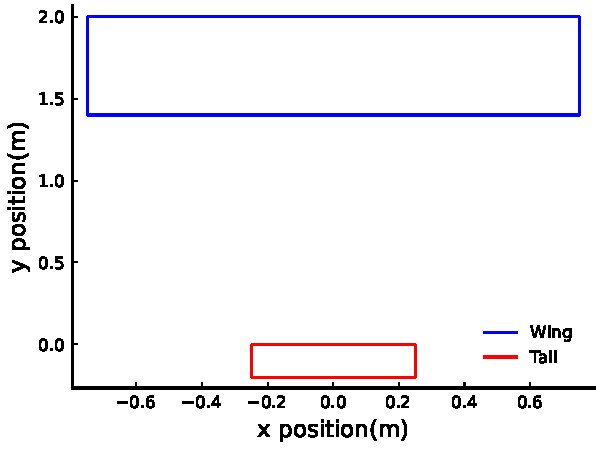
\includegraphics{../graphics/chord_design.pdf}
		\caption{\emph{The design of an airframe with a chord length of 0.6 m.}}
		\label{fig:chord_design}
	\end{figure}
	
	An airframe with a greater chord length was not evaluated for comparison, because of the constraint I put on the aspect ratio. 0.7222 m was the largest possible chord length that kept the aspect ratio of the wing greater than 2.0.\\
	
	Plots showing the lift coefficient vs. angle of attack and drag coefficient vs. angle of attack for these 2 designs are given (see figure \ref{fig:chord_coeff}).
	
	\begin{figure}[H]
		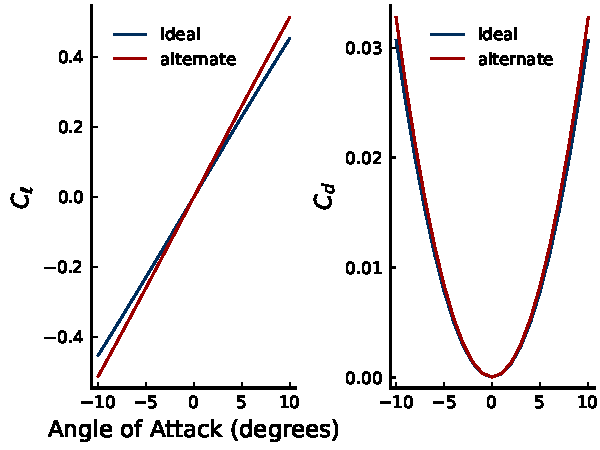
\includegraphics{../graphics/chord_coeff.pdf}
		\caption{\emph{The lift and drag coefficients for varying angles of attack for the 2 designs evaluated using different mean chord lengths.}}
		\label{fig:chord_coeff}
	\end{figure}
	
	When evaluating an airframe that has a length from wing to tail that is less than 2.0 m (I used 1.0 m), it was found that the velocity needed to generate the necessary lift does not change. However, the airframe is less stable as the yaw stability derivative(\(C_{nb}\)) is less than the yaw stability derivative for the optimized airframe. Therefore, as the length from wing to tail is decreased, the airframe becomes less stable.\\
	
	Figures showing the lift and drag coefficients vs. angle of attack for the 2 designs are given (see figure \ref{fig:wingtail_coeff}). 
	
	\begin{figure}[H]
		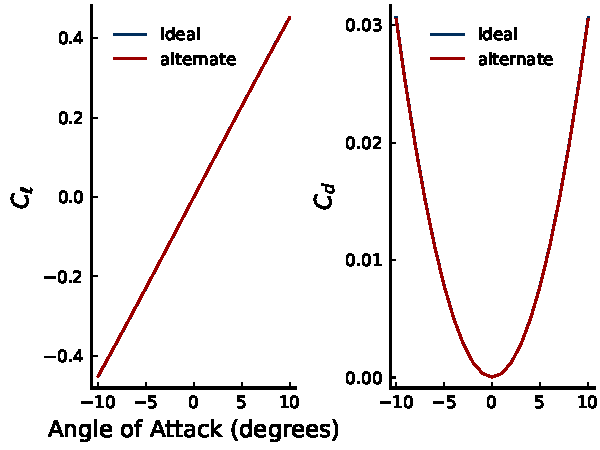
\includegraphics{../graphics/wingtail_coeff.pdf}
		\caption{\emph{The lift and drag coefficient vs. angle of attack for the 2 designs evaluated.}}
		\label{fig:wingtail_coeff}
	\end{figure}
	
	Figure \ref{fig:length_design} shows the design of an airframe with a length from wing to tail of 1.0 m.
	
	\begin{figure}[H]
		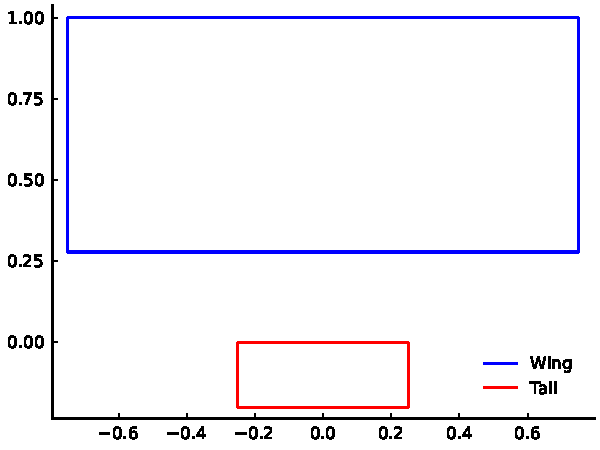
\includegraphics{../graphics/length_design.pdf}
		\caption{\emph{The design of an airframe with a length from wing to tail of 1.0 m.}}
		\label{fig:length_design}
	\end{figure}
	
	The wing taper ratio of an airframe is found using equation \ref{eqn:taper-ratio}.
	
	\begin{equation}
		Taper\ Ratio = \frac{tip\ chord\ length}{base\ chord\ length}
		\label{eqn:taper-ratio}
	\end{equation}
	
	When evaluating an airframe that has a wing taper ratio that is less than 1.0 (I used 0.5), it was found that the velocity needed to calculate the necessary lift was 13.215339717762241 m/s. While this is close to the velocity needed for the optimized airframe, it is still larger; therefore, it is not as optimal. This shows that as the wing taper ratio is decreased, the velocity needed to lift 0.5 kilograms increases, making it sub-optimal. You can also see that an airframe with a wing taper ratio of 1.0 has a lift coefficient distribution that is closer to the optimal elliptical distribution than the airframe with a wing taper ratio of 0.5 (see figures \ref{fig:cl_dist} and \ref{fig:cl_dist_compare}).\\
	
	\begin{figure}[H]
		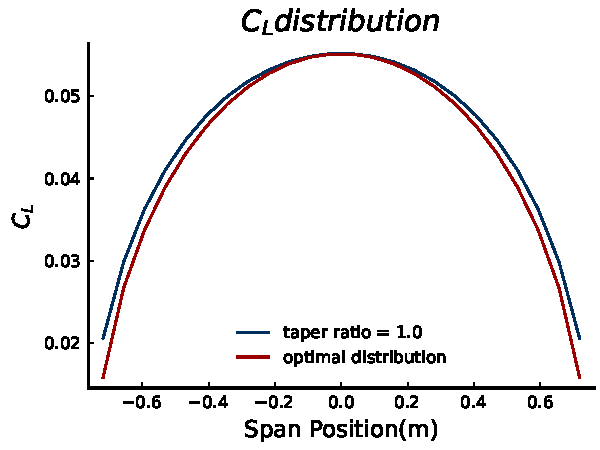
\includegraphics{../graphics/cl_dist.pdf}
		\caption{\emph{The lift coefficient distribution for a taper ratio of 1.0 vs. the optimal elliptical distribution.}}
		\label{fig:cl_dist}
	\end{figure}
	\begin{figure}[H]
		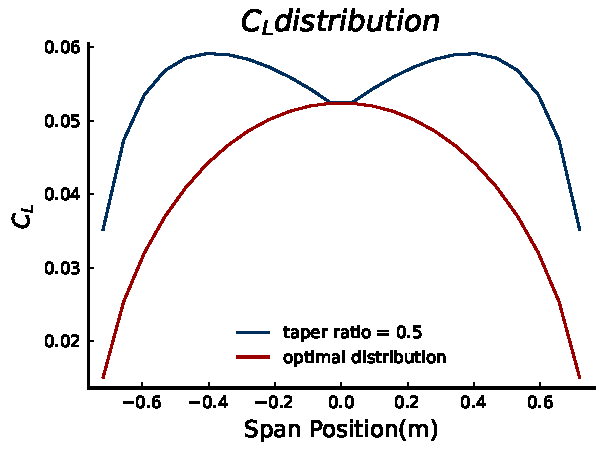
\includegraphics{../graphics/cl_dist_compare.pdf}
		\caption{\emph{The lift coefficient distribution for a taper ratio of 0.5 vs. the optimal elliptical distribution.}}
		\label{fig:cl_dist_compare}
	\end{figure}
	
	Plots showing the lift coefficients and drag coefficients vs. angle of attack for these 2 designs are given (see figure \ref{fig:taper_coeff}).
	
	\begin{figure}[H]
		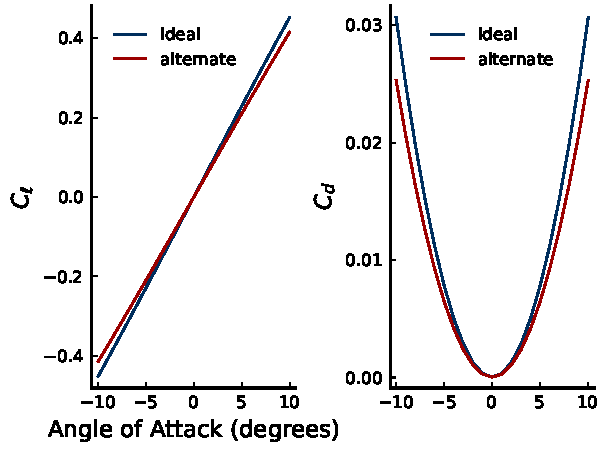
\includegraphics{../graphics/taper_coeff.pdf}
		\caption{\emph{The lift and drag coefficients for varying angles of attack for the 2 designs evaluated using different wing tip tapers}}
		\label{fig:taper_coeff}
	\end{figure}
	
	The design of an airframe with a wing taper ratio of 0.5 is shown in figure \ref{fig:taper_design}.
	
	\begin{figure}[H]
		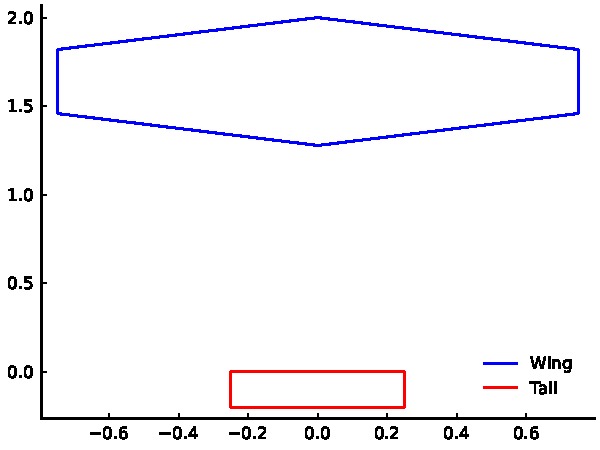
\includegraphics{../graphics/taper_design.pdf}
		\caption{\emph{The design of an airframe with a wing taper ratio of 0.5.}}
		\label{fig:taper_design}
	\end{figure}

	\section{Conclusion}
	By designing an actual airframe using the skills and knowledge gained from the research done on airfoils and airframes, I learned valuable insights. One of the more important things I learned from optimizing the airframe was that when writing computer programs to solve optimization problems, it is important to make sure that the program accounts for realistic outputs. In the case of optimizing an airframe, I had to put constraints on the aspect ratio so that the mean aerodynamic chord length was a realistic value. If I hadn't done that, the program would have outputted an airframe with the max chord length possible, because mathematically, that is optimal. I also learned that there is a plethora of design variables that can be altered when designing an airframe, which makes it important to only alter a few at a time to be able to see their effects better. From the research on airfoils and airframes, I learned about what effects airfoil polar, how to use tools such as Xfoil.jl \cite{McDonnell} and VortexLattice.jl \cite{McDonnell-Ning} to evaluate airfoils and airframes, and how those tools compare to acctual experimental data.\\
 	
 	\printbibliography
	
\end{document}